%%%%%%%%%%%%%%%%%
%% BASIC SETUP %%
%%%%%%%%%%%%%%%%%
\documentclass[12pt]{article}

% Necessary packages
\usepackage{titling}
\usepackage{geometry}
\usepackage{mathptmx}
\usepackage{hyperref}
\usepackage{booktabs}
\usepackage{float}
\usepackage{graphicx}
\usepackage{titlesec}
\usepackage{setspace}
\usepackage{lscape}
\usepackage[tableposition=top]{caption}

% Title page margins
\newgeometry{top=2in, bottom=1in, left=1.5in, right=1.5in}

% Define commands to switch margins
\newcommand{\titlepagegeometry}{\newgeometry{top=2in, bottom=1in, left=1.5in, right=1.5in}}
\newcommand{\documentgeometry}{\newgeometry{top=1in, bottom=1in, left=1in, right=1in}}

% Table of contents formatting
\setcounter{secnumdepth}{3}

% General caption setup
\captionsetup{width=1\textwidth}

% Custom label format for figures
\DeclareCaptionLabelFormat{bold}{\textbf{#1~#2}}

% Figure caption setup
\captionsetup[figure]{
  format=plain, 
  justification=centering,
  labelformat=bold,  
  labelsep=period
}

% Table caption setup
\captionsetup[table]{
  labelfont=bf,
  labelsep=period,
  position=top,
}

% Footnote formatting
%\newcommand{\smallerfootnotes}{\footnotesize}

% Spacing
\setlength{\parskip}{1.5em}

% Adjust spacing for section and subsection headings
\titlespacing*{\section}{0pt}{*0}{*0}
\titlespacing*{\subsection}{0pt}{*0}{*0}
\titlespacing*{\subsubsection}{0pt}{*0}{*0}

\begin{document}


%%%%%%%%%%%%%%%%%
%% TITLE PAGE %%
%%%%%%%%%%%%%%%%%
\begin{titlepage}
    \centering
    \vspace*{-3cm}
    
\includegraphics[width=0.5\textwidth]{reports/unc-logo.png}\par
    \vspace{0.5cm}
    {\Huge\bfseries Investigating Reasons for Uninsurance in the 2023 U.S. National Health Interview Survey \par}
    \vspace{2cm}
    {\LARGE Julia G. Muller\par}
    {\Large Gillings School of Global Public Health \par}
    {\Large University of North Carolina at Chapel Hill \par}
    \vspace{3cm}
    {\large A final capstone submitted for the Master of Public Health in Applied Epidemiology \par}
    \vspace{1cm}
    {\large 15 April 2025\par}
    \vspace{1cm}
\end{titlepage}


%%%%%%%%%%%%%%%%%%%%%%%
%% TABLE OF CONTENTS %%
%%%%%%%%%%%%%%%%%%%%%%%
\newpage
\documentgeometry
\tableofcontents


%%%%%%%%%%%%%%%%%%
%% INTRODUCTION %%
%%%%%%%%%%%%%%%%%%
\newpage
\section{Introduction}

Among industrialized nations, the United States spends twice as much on healthcare as the median nation while having one of the worst qualities of healthcare (Davis, 2007). The US is one of the only industrialized nations without universal health insurance. People who do not have insurance face increased financial burden, barriers in access to care, lost economic productivity, and worse patient outcomes (Davis, 2007). Studies have found that people who have insurance have more statistically significant positive health outcomes in general health, general physical functioning, mortality, health disease, cancer, diabetes, and acute conditions (McWilliams, 2009). In terms of financial burden, 49\% of uninsured adults report difficulty paying medical bills, compared to only 21\% of individuals with private insurance, and a higher percentage of uninsured adults report having medical debt (Tolbert, 2024). Uninsured status also restricts access to preventative care and health care services – people without insurance are more likely to delay or forgo medical care because of costs (Cha \& Cohen, 2020). Not having insurance can also have downstream effects on a person’s ability to access specialized healthcare resources. For example, participants who were disenrolled in a Washington State AIDS Drug Assistance Program between 2017 and 2019 were more likely to be uninsured compared to those with private insurance, despite insurance not being a requirement for the program (Erly et al., 2022). For these reasons, addressing remaining insurance gaps is critical to ensure equitable access to health care and positive health outcomes. Despite the expansion of the Affordable Care Act, many people remain uninsured (Tolbert et al., 2024). Understanding the reasons why people remain uninsured, and the impact of those reasons on the length of time they go without insurance, could identify potential avenues for interventions to close the uninsurance gap.

As of 2023, an estimated 21.3 million individuals aged 18-64 were uninsured (Tolbert et al., 2024). The percentage of adults in the US aged 18-64 who were uninsured vary across different demographics, with a higher prevalence among racial and ethnic minorities (Lee et al. 2021). In 2018, uninsured working-age adults in the US were found to be disproportionately low income, Latino, and under the age of 25 (Collins \& Gunja, 2019). Additionally, the reasons for uninsurance differ by demographic factors. In 2023, 63\% of adults aged 18-64 claimed that the high cost of insurance as the main reason they are uninsured (Tolbert et al., 2024). High cost of care as the primary barrier increases with age from 66.8\% among those aged 18-29 to 80.9\% for those aged 50-64 (Cha \& Cohen, 2020). Hispanic adults were also more likely to be uninsured due to issues about eligibility (Cha \& Cohen, 2020). Men were more likely than women to not have insurance because it was not needed or wanted (Cha \& Cohen 2020). Those who were uninsured were more likely to be non-Hispanic black or Hispanic, have less than a high school education, and have an annual household income less than \$35,000 (Okoro et al., 2015). Investigating the different reasons among the varying demographics of those uninsured is paramount to finding adequate interventions that are suited to helping the specific demographic groups that need it.

From our literature review, most studies about insurance included adults aged 18-64. Individuals under 18 can be included in their parents’ insurance, and additional federal support programs, such as the Children’s Health Insurance Program (CHIP), are available and adults over the age of 18 are more likely to be uninsured than children (Tolbert et al., 2024; U.S. Centers for Medicare \& Medicaid Services, n.d.-a). However, studies show that children in the US can also suffer from inconsistent or no insurance with 34\% of US children in 2019 suffering from this (Daw et al. 2023). Additionally, individuals ages 65 and older are also excluded from most studies because they are automatically eligible for Medicare, which offers a no-cost Part A insurance (U.S. Centers for Medicare and Medicaid Services, n.d.-b). Therefore, there should effectively be no uninsured adults over 65. However, there are still some papers that address this assumption, and document the gaps in insurance coverage for this older demographic (Mold et al., 2004). The contextual factors of studies are crucial to this topic, as insurance policy changes with time, location, and individual age. Several of the previous studies on this topic were done before the implementation of the Affordable Care Act (ACA) in 2010. In later studies, it is important to consider the time and location of the study, as states choose to expand Medicaid at different times. Some studies are stratified between different periods after the ACA, such as the implementation period between 2010-2013 and the expansion of Medicaid and Marketplaces between 2014-2016 (Wisk \& Sharma, 2019). Additionally, different insurance plans are available for different income levels and age groups.

Further study of reasons for being uninsured is needed, as expansion of ACA and the COVID-19 pandemic both impacted insurance coverage availability in the United States. While the ACA led to gains in health insurance coverage, substantial gaps remain. Gains in Marketplace use and Medicaid coverage in the expansion period of 2014 to 2016 were found among young adults 19-30 years of age, but disparities remained among female, lower socioeconomic status, non-citizens, non-English speakers, and several racial/ethnic minority groups (Wisk \& Sharma, 2019). These racial and ethnic disparities in health insurance coverage were found to be exacerbated by the COVID-19 pandemic (Freelander et al., 2023). Additionally, we found very few papers that looked at geographic factors such as urban-rural location or region of the United States. While we found many studies examining insurance coverage, relatively few examined the specific reasons for being uninsured. Furthermore, we found no studies specifically linking the reasons for not having health insurance with the duration of uninsurance. The goal of this study is to explore the reasons for not having insurance among adults, ages 18-64, who are not insured. By stratifying by various demographic and geographic characteristics, our study will also examine whether these reasons change among different populations.


%%%%%%%%%%%%%
%% METHODS %%
%%%%%%%%%%%%%
\newpage
\section{Methods}

Data were obtained from the 2023 National Health Interview Survey, a nationally representative cross-sectional survey of the non-institutionalized U.S. population. All respondents were asked whether they currently had health insurance. Those who answered that they did not, were asked further questions about reasons for no insurance and duration without coverage.

Our target population is uninsured adults between the ages of 18 and 64 in the United States. These adults are not eligible for Medicare, which starts at 65 years of age. In order for individuals to be included in our study, they must be ages 18-64 and be uninsured at the time of the survey. This includes not having Medicare, Medicaid, any non-Medicaid state-sponsored health insurance program, CHAMPUS, CHAMPVA coverage, or any private insurance. Individuals who have any of these insurance plans were not included in the study. Our final study population consisted of 1,937 individuals.

Our primary exposure variable was the reasons a person does not have insurance. Uninsurance is defined as having no insurance or persons with a single service plan. The response options include: unemployment, high cost, not wanting insurance, plans not meeting needs, coverage has not started yet, missed deadline, or other reasons (not provided by the interviewer). Our primary outcome variable was time since the respondent last had health insurance, among those who were uninsured at the time of the survey. Responses were grouped by NHIS into the following categories: less than 1 year, 1 year to less than 2 years, 2 years to less than 3 years, 3 years or more, less than 5 years, 5 years or more, less than 10 years, 10 years or more, never, and unknown (refused, not ascertained, don’t know). The reasons for unknown were originally separated by NHIS, but we combined them due to small sample size. We additionally examined sociodemographic variables, including self-reported race, self-reported Hispanic, Spanish, or Latino origin or ancestry, urban or rural residence (large central metro, large fringe metro, medium- and small-metro county, or non-metro county), age in years, sex as identified by interviewer, and highest level of education completed.

For measures of occurrence, the prevalence of each reason why an individual does not have insurance was calculated in total and across covariates (race, ethnicity, urban/rural status, sex, level of education). Additionally, we calculated descriptive statistics for the duration of uninsurance, including the total average duration and average duration for each reason. 

For our analysis, we looked at the difference in the frequency distribution of reasons by different durations of time without insurance. Then, we used ANOVA to look for correlation between duration and reasons for no insurance. We used a chi-squared test to test if the difference in duration without insurance is significantly different between reasons for not having insurance. We also assessed differences in proportions across different covariate strata, including urban vs rural, race, and ethnicity. Analyses were performed in SAS and R.

For this study, our sample is a large and comprehensive group analyzing people in the United States who do not have health insurance across major socio-demographic groups. The results can be largely generalized across the country. This generalizability is due to the number of covariates included in the study, providing a comprehensive outlook on race and ethnic categories, urban and rural differences, educational attainment, age distributions, and differences in sex. This large number of covariates allowed us to adjust for potential confounders. As we excluded children under 18 years old who mostly have insurance through their parents and adults over 65 years old who mostly have insurance through Medicare, selection bias is mitigated in our age covariates. However, there is the possibility of selection bias if people who do not have insurance are less likely to respond to the survey. In this case, this study will only be looking at people who respond to the survey, and not necessarily an accurate representation of demographics in the United States. Furthermore, this study is cross-sectional, meaning we cannot establish temporality between reasons for uninsurance and duration of uninsurance and have limited ability to make causal inferences.



%%%%%%%%%%%%%
%% RESULTS %%
%%%%%%%%%%%%%
\newpage
\section{Results}

% Table 1
\newpage
\begin{table}[H]
  \vspace*{-1.5cm}
  \hspace*{-1cm} 
  \centering
  \rotatebox{90}{
\includegraphics[width=24cm]{figures/table_1.png}}
  \caption{Demographic characteristics}
\end{table}

% Table 2
\newpage
\begin{table}[H]
  \vspace*{0cm}
  \hspace*{-1.75cm} 
  \centering
  \rotatebox{90}{
\includegraphics[width=22cm]{figures/table_2.png}}
  \caption{idk yet}
\end{table}

% Distribution of duration without insurance
\begin{figure}[H]
  \centering
  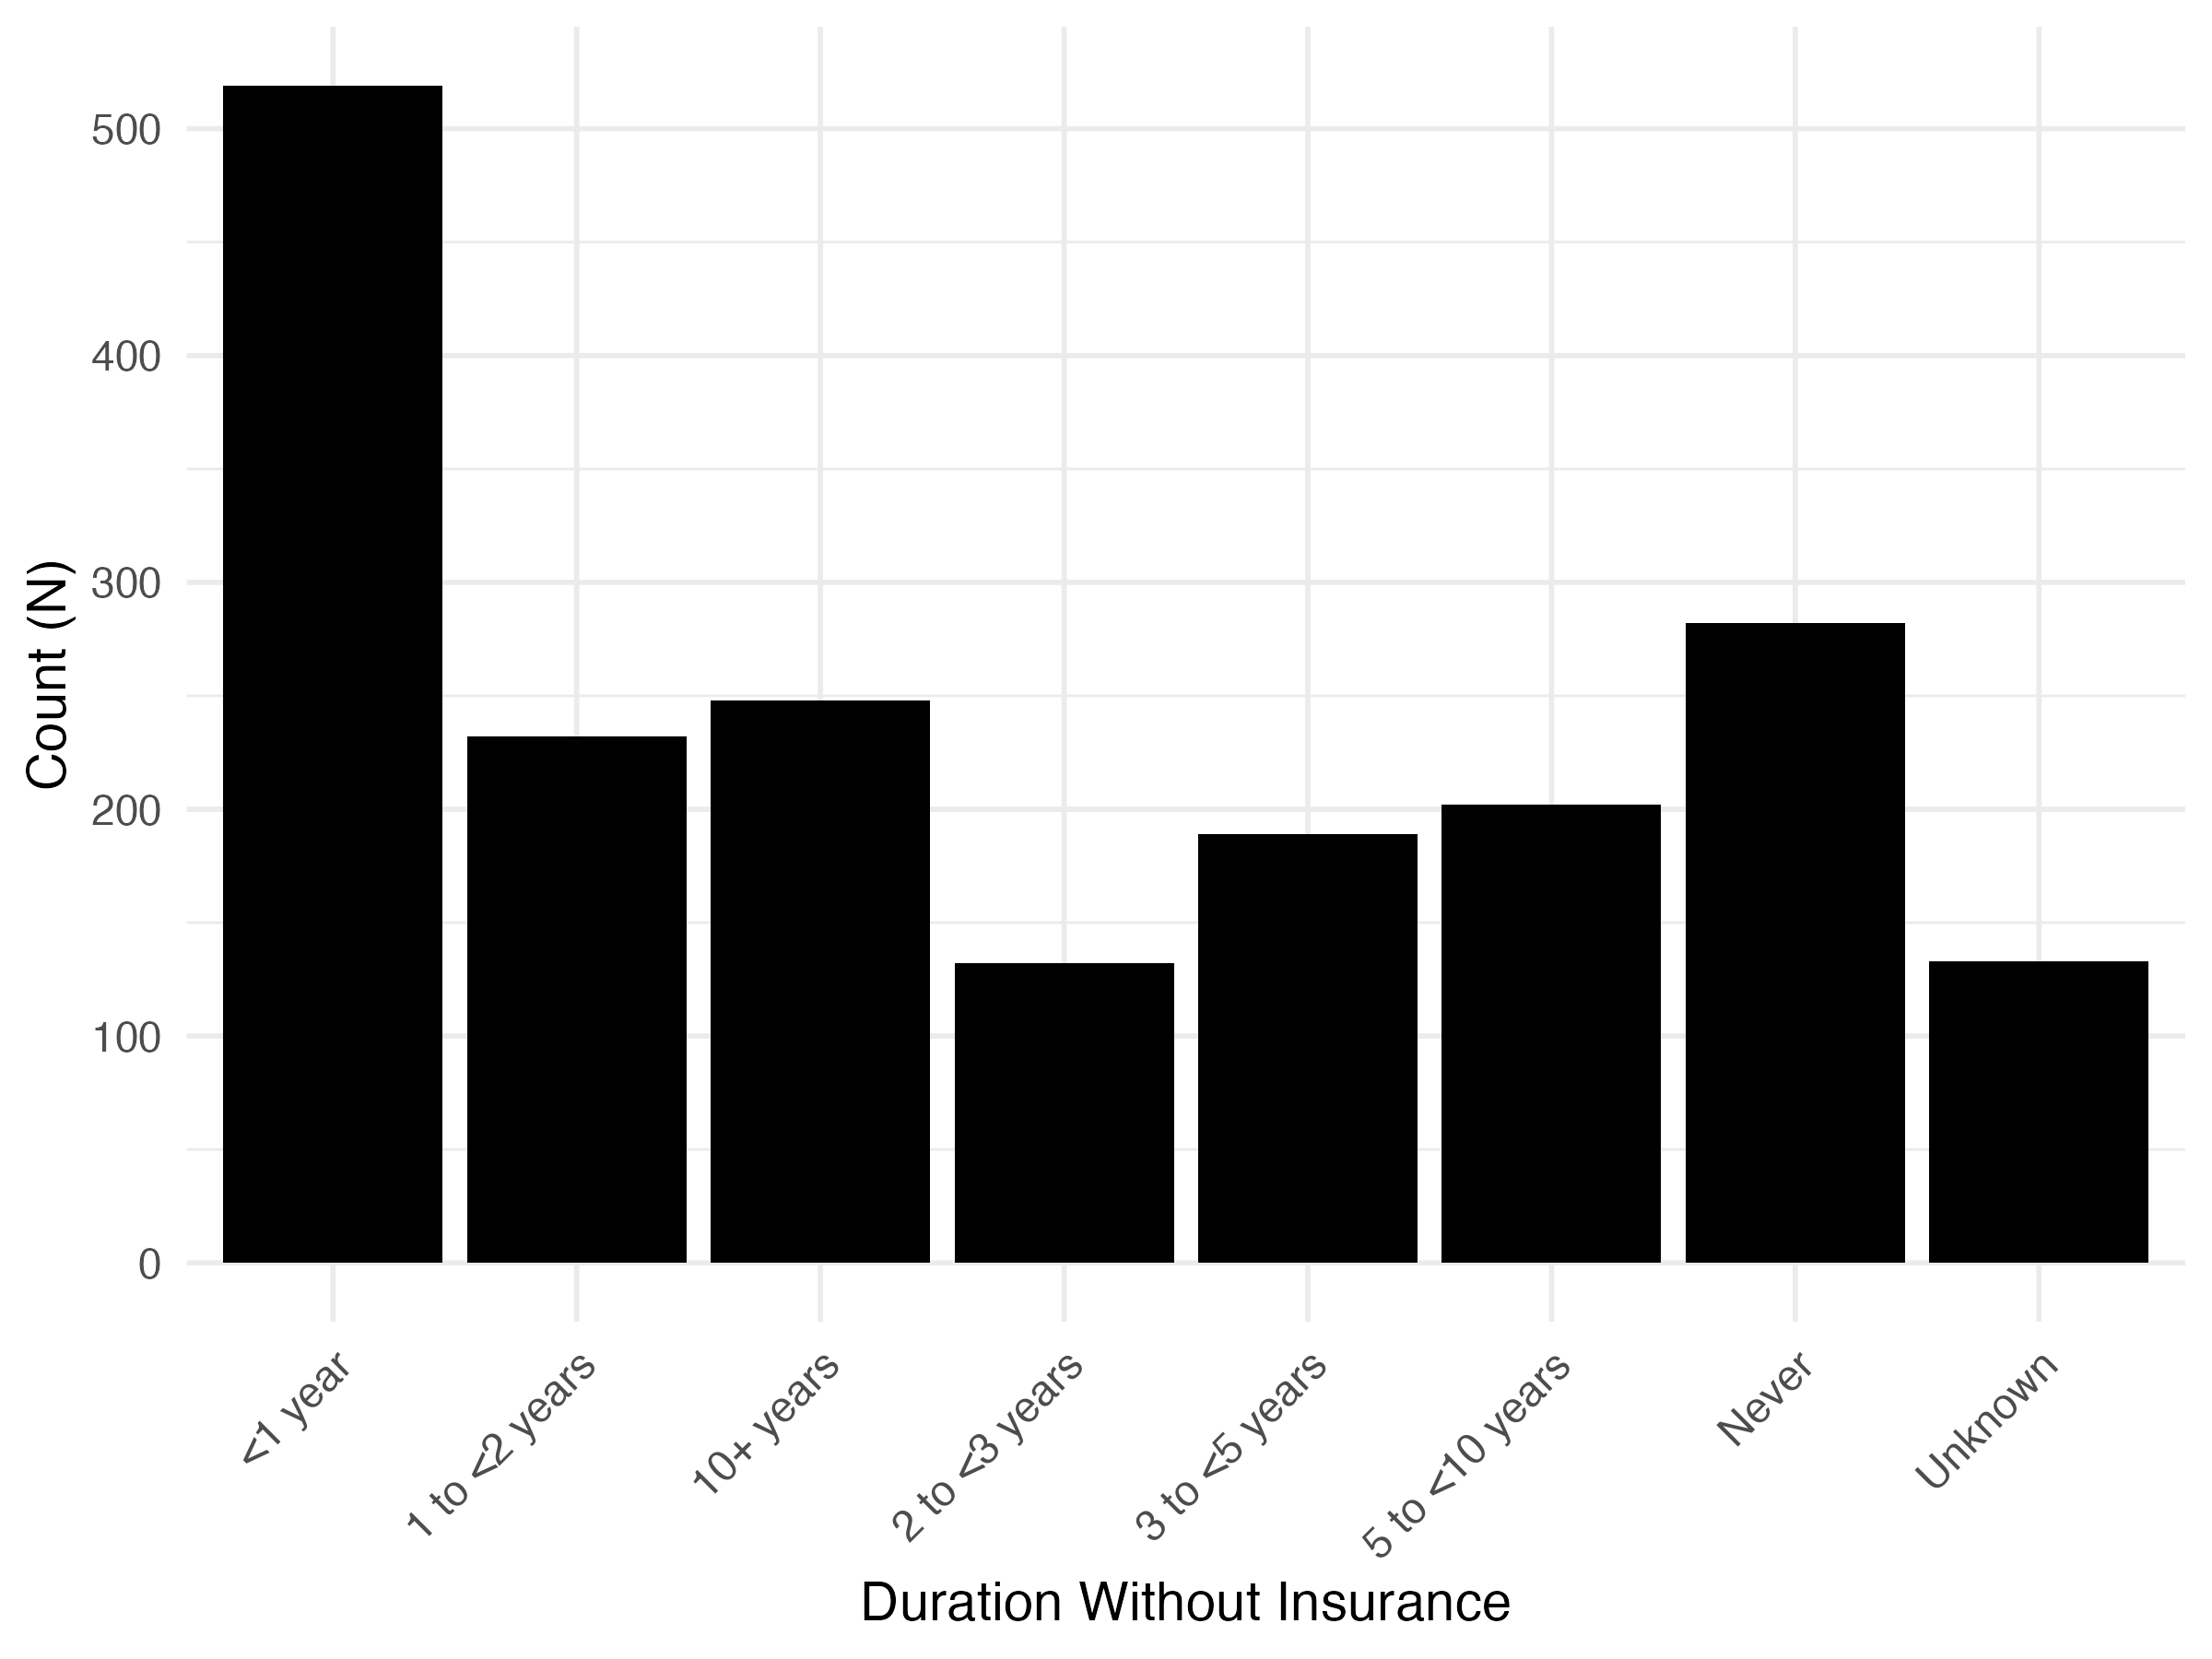
\includegraphics[width=15cm]{figures/duration_no_insurance.png}
  \caption{Distribution of duration without insurance.}
\end{figure}

% Line graph of duration without insurance by reason
\begin{figure}[H]
  \centering
  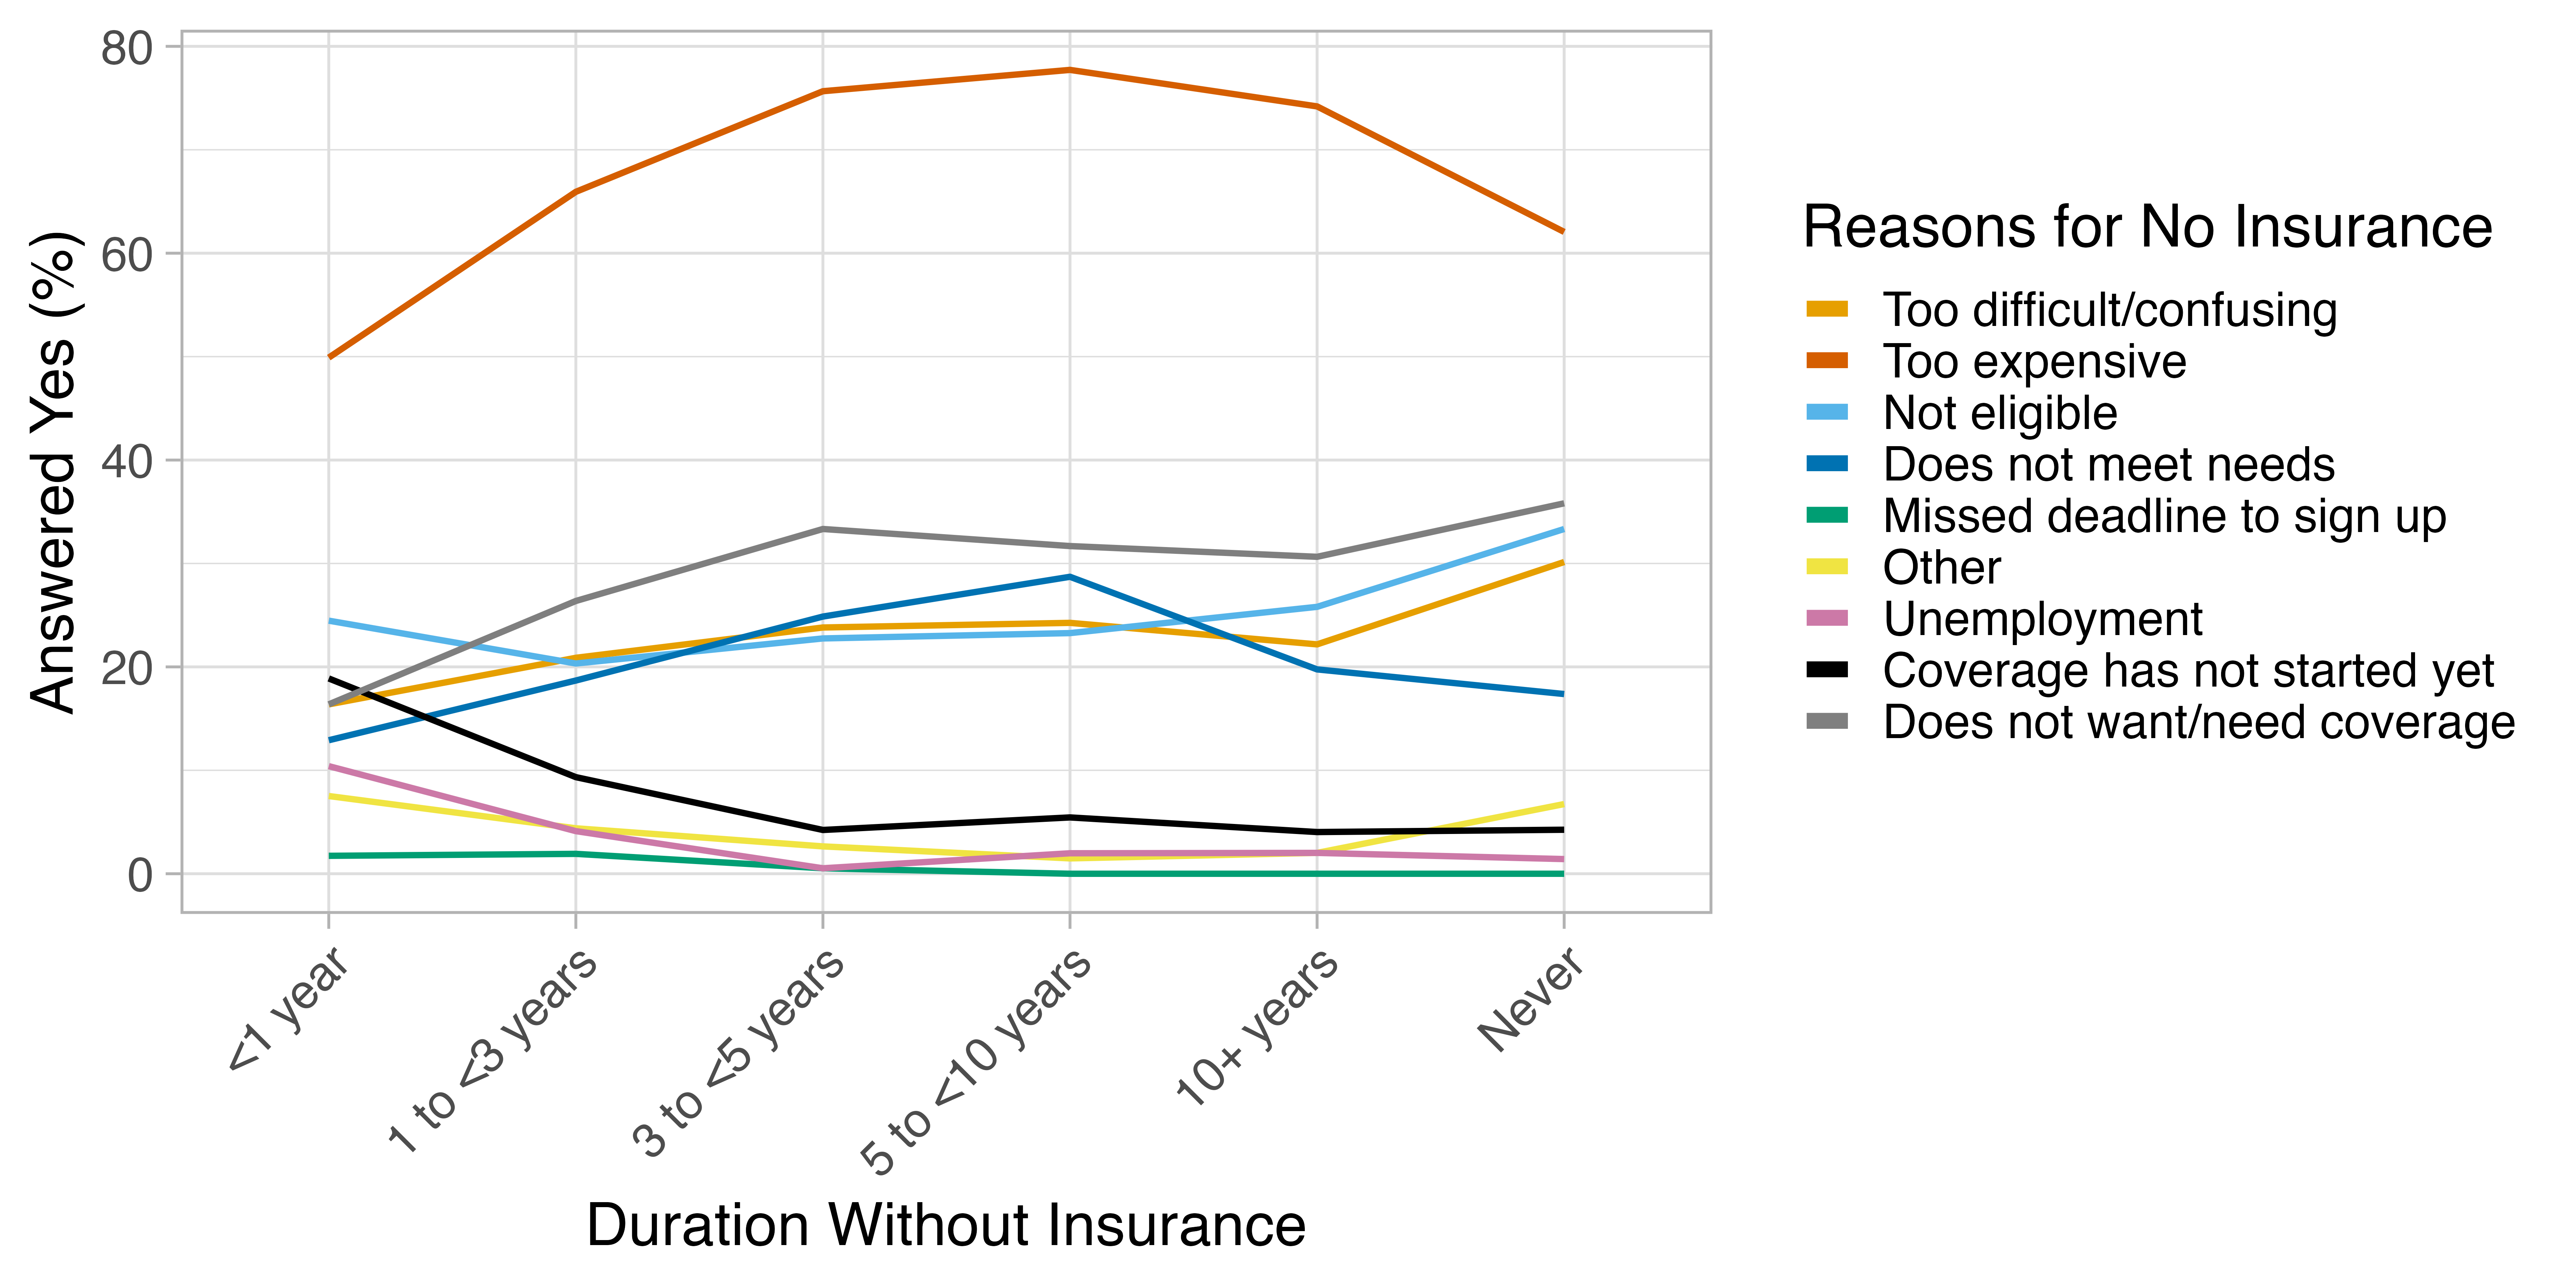
\includegraphics[width=18cm]{figures/duration_no_insurance_by_reason.png}
  \caption{Line graph of duration without insurance for each reason.}
\end{figure}


%%%%%%%%%%%%%%%%
%% DISCUSSION %%
%%%%%%%%%%%%%%%%
\newpage
\section{Discussion}


\end{document}